\documentclass[aps,pre,reprint,superscriptaddress,longbibliography,floatfix]{revtex4-2}

\usepackage{amsmath,amssymb,bm}
\usepackage{graphicx}
\usepackage{physics}
\usepackage{hyperref}

% Custom commands
\newcommand{\Ms}{\mathcal{M}}
\newcommand{\Ds}{\mathcal{D}}
\newcommand{\Cs}{\mathcal{C}}
\newcommand{\Ks}{\mathcal{K}}
\newcommand{\Da}{\mathrm{Da}}
\newcommand{\Bi}{\mathrm{Bi}}
\newcommand{\Pe}{\mathrm{Pe}}
\newcommand{\Rhat}{\widehat{R}}
\newcommand{\pp}{\phi_{p0}}

\begin{document}

\title{Reaction-Driven Self-Oscillation in Thermoresponsive Gels: \\
From Bifurcation Analysis to Geometry-Dependent Dynamics}

\author{Author}
\affiliation{Affiliation}

\date{\today}

\begin{abstract}
Thermoresponsive hydrogels with lower critical solution temperature (LCST)
can exhibit self-sustained volume oscillations when coupled to an
exothermic chemical reaction. We develop a hierarchy of models---from a
lumped zero-dimensional (0D) system to spatially resolved one-dimensional
(1D) slab and spherical geometries---to elucidate the oscillation
mechanism and its dependence on geometry. The 0D model identifies Hopf
bifurcation boundaries in the Damk\"ohler number $\Da$ and LCST
sensitivity $S_\chi$ parameter space, predicting two oscillatory
regimes: a large-amplitude relaxation oscillator (Regime~I) and a
small-amplitude near-harmonic oscillator (Regime~II). The 1D slab model
reveals the spatial structure of these oscillations, including a
dual-zone termination mechanism in which the outer shell is shut off by
accessibility collapse while the inner core is limited by reactant
depletion. Crucially, we show that geometry plays a decisive role:
the slab geometry sustains robust oscillations, whereas the spherical
geometry suppresses them due to enhanced radial solvent influx and, in
the full-mechanics case, anisotropic stress locking. Finally, we
demonstrate that reactant penetration depth can be enhanced more than
$590\times$ by optimizing the $\Da$--$D_0$--$\Bi_c$ parameter
combination, providing design guidelines for autonomous
chemical-delivery applications.
\end{abstract}

\maketitle

%% ================================================================
%%  I. INTRODUCTION
%% ================================================================
\section{Introduction}
\label{sec:intro}

Stimuli-responsive gels that undergo spontaneous, self-sustained volume
oscillations have attracted attention as minimal models of biological
rhythms and as candidate components for soft actuators, chemical
oscillators, and autonomous drug-delivery
systems~\cite{Yoshida2010,Yashin2006}. The most studied synthetic
realization couples a thermoresponsive network---typically based on
poly($N$-isopropylacrylamide) (PNIPAM) with a lower critical solution
temperature (LCST) around $33\,^\circ\mathrm{C}$---to an oscillatory or
exothermic chemical reaction such as the Belousov--Zhabotinsky (BZ)
reaction~\cite{Yoshida2002,Yoshida2004}. In these systems, chemical
oxidants produced by the BZ reaction swell the gel, while reductants
cause collapse; the gel's spatiotemporal dynamics feed back on the local
oxidant concentration, giving rise to autonomous
oscillation~\cite{Yashin2006}.

A complementary oscillation route, less well studied, relies on purely
\emph{thermal} feedback: an exothermic reaction heats the gel above the
LCST, the attendant volume collapse expels solvent and reactant, the gel
cools, swells again, and re-ingests fresh reactant---completing one
cycle. This thermo-mechanical-chemical feedback loop does not require
multi-step BZ chemistry; a single irreversible exothermic reaction
suffices. Early theoretical work by Siegel and coworkers demonstrated
this concept for spherical gel beads~\cite{Siegel1988,Siegel1992}, and
subsequent studies identified parameter regimes of self-oscillation in
slab and membrane geometries~\cite{Zarzycki2020,Boissonade2003}.
However, several fundamental questions remain open:
\begin{enumerate}
  \item What are the minimal conditions---expressed in terms of
    dimensionless groups---for the thermal oscillation to occur?
  \item How does the spatial structure of the gel affect the oscillation
    mechanism, and what role does geometry (slab vs.\ sphere) play?
  \item Can the oscillation be harnessed for practical applications
    such as periodic chemical delivery, and if so, what parameters
    maximize interior reactant penetration?
\end{enumerate}

In this paper, we address these questions through a systematic hierarchy
of models:
\begin{itemize}
  \item An \emph{analytical linear-stability analysis of the 1D slab}
    (Sec.~\ref{sec:0d}) that derives the dispersion relation, identifies
    the Hopf window, and separates long-wave oscillatory instability
    from finite-wavenumber spinodal growth.
  \item A \emph{1D slab model} (Sec.~\ref{sec:slab}) that resolves
    spatial gradients and reveals the oscillation mechanism, including
    two distinct regimes and a dual-zone termination mechanism.
  \item A \emph{1D sphere model} (Sec.~\ref{sec:geometry}) that
    demonstrates how radial geometry suppresses oscillation via enhanced
    solvent transport and anisotropic stress effects.
  \item A \emph{penetration optimization study}
    (Sec.~\ref{sec:penetration}) that provides quantitative design
    guidelines for maximizing interior reactant delivery.
\end{itemize}

The model integrates large-deformation poroelastic mechanics
(Flory--Rehner free energy), heat diffusion with exothermic reaction
source, and reactant transport coupled to the local swelling state. The
dimensionless formulation reduces the parameter space to eight key
groups, facilitating systematic exploration. Full derivations and
numerical details are given in
Appendices~\ref{app:model}--\ref{app:numerics}.


%% ================================================================
%%  II. MODEL FORMULATION
%% ================================================================
\section{Model Formulation}
\label{sec:model}

\subsection{Physical system}

We consider a thermoresponsive gel body containing an immobilized
catalyst that catalyzes an exothermic, irreversible reaction consuming a
substrate (reactant) supplied by the surrounding bath. Two geometries are
studied: (i)~a \emph{symmetric slab} of dry-state half-thickness $H_0$,
with Lagrangian coordinate $\xi=X/H_0\in[0,1]$; and (ii)~a
\emph{sphere} of dry-state radius $R_0$, with radial coordinate
$s=R/R_0\in[0,1]$. In both cases, $\xi=0$ (or $s=0$) is the symmetry
center and $\xi=1$ (or $s=1$) is the free surface.

\subsection{Governing equations}

The three primary fields are the local swelling ratio $J$, the normalized
reactant concentration $u$ (scaled by the bath value), and the
dimensionless temperature excess $\theta=(T-T_0)/\Delta T_\mathrm{ref}$.
The dimensionless governing equations (derived in
Appendix~\ref{app:nondim}) are
\begin{subequations}
\label{eq:governing}
\begin{align}
  \frac{\partial J}{\partial t} &= -\frac{\partial}{\partial \xi}
    \Bigl[\Ms(J)\,\frac{\partial\mu}{\partial\xi}\Bigr], \label{eq:gov_J}\\[4pt]
  \frac{\partial (uJ)}{\partial t} &= \frac{\partial}{\partial\xi}
    \Bigl[\Ds(J)\,\frac{\partial u}{\partial\xi}\Bigr]
    - \Da\,J\,\Rhat(u,J,\theta), \label{eq:gov_u}\\[4pt]
  \Cs(J)\,\frac{\partial\theta}{\partial t} &= \frac{\partial}{\partial\xi}
    \Bigl[\Ks(J)\,\frac{\partial\theta}{\partial\xi}\Bigr]
    + \Da\,J\,\Rhat(u,J,\theta), \label{eq:gov_theta}
\end{align}
\end{subequations}
where $\Ms$ is the swelling mobility, $\Ds$ and $\Ks$ are the effective
reactant diffusivity and thermal conductivity, and $\Cs$ is the effective
heat capacity. The reaction rate is
\begin{equation}
  \Rhat = u\,(1-\phi)^{m_\mathrm{act}}\,
  \exp\!\Bigl(\frac{\Gamma_A\,\theta}{1+\varepsilon_T\,\theta}\Bigr),
  \label{eq:rxn}
\end{equation}
with $\phi = \pp/J$. The solvent chemical potential $\mu[J,\theta]$ is
derived from the Flory--Rehner free energy with a temperature-dependent
$\chi$ parameter exhibiting an LCST transition
(Appendix~\ref{app:model}).

For the spherical geometry, the Laplacian in
Eqs.~\eqref{eq:governing} acquires the factor $(1/s^2)\partial_s(s^2
\cdot)$, and the elastic contribution to $\mu$ includes anisotropic
stretch corrections (Appendix~\ref{app:model}).

\subsection{Boundary conditions}

At the symmetry center ($\xi=0$ or $s=0$), all fluxes vanish. At the
free surface ($\xi=1$ or $s=1$):
\begin{equation}
  \mu\big|_{\xi=1}=0,\quad
  \Ds\,\frac{\partial u}{\partial\xi}\Big|_{\xi=1}=\Bi_c\,(1-u),\quad
  \Ks\,\frac{\partial\theta}{\partial\xi}\Big|_{\xi=1}=-\Bi_T\,\theta.
  \label{eq:bc}
\end{equation}

\subsection{Lumped (0D) model}

The spatially uniform limit yields a three-ODE system for $J(t)$,
$u(t)$, $\theta(t)$, where surface exchange enters through Biot-number
terms:
\begin{subequations}
\label{eq:0d}
\begin{align}
  \dot{J}  &= \Bi_\mu\,J^{2/3}\bigl[\mu_b - \mu(J,\theta)\bigr],
    \label{eq:0d_J}\\
  \frac{d(Ju)}{dt} &= \Bi_c\,J^{2/3}(1-u) - \Da\,J\,\Rhat,
    \label{eq:0d_u}\\
  \Cs(J)\,\dot\theta &= \Da\,J\,\Rhat - \Bi_T\,J^{2/3}\,\theta.
    \label{eq:0d_theta}
\end{align}
\end{subequations}
This system is amenable to standard bifurcation analysis and provides
analytical insight into the oscillation mechanism.

\subsection{Dimensionless parameters}

The eight control parameters are summarized in Table~\ref{tab:params}.

\begin{table}[h]
\centering
\caption{Key dimensionless parameters.}
\label{tab:params}
\begin{ruledtabular}
\begin{tabular}{clcc}
Symbol & Physical meaning & Default & Range\\
\hline
$\Da$            & Reaction / diffusion rate      & 4     & 3--18\\
$\Bi_c$          & Surface reactant exchange      & 0.70  & 0.1--2\\
$\Bi_T$          & Surface heat loss              & 0.10  & 0.05--0.5\\
$S_\chi$         & LCST sensitivity               & 1.0   & 0.5--8\\
$\Gamma_A$       & Arrhenius sensitivity           & 1.5   & 0--7\\
$D_0$            & Reactant diffusivity scale     & 2.0   & 0.5--3\\
$m_\mathrm{act}$ & Reaction accessibility exponent& 6     & 1--6\\
$m_\mathrm{diff}$& Diffusion tortuosity exponent  & 2     & 1--6\\
\end{tabular}
\end{ruledtabular}
\end{table}


%% ================================================================
%%  III. LINEAR STABILITY OF THE 0D MODEL
%% ================================================================
\section{Linear Stability of the 1D Slab}
\label{sec:0d}

Before turning to the fully nonlinear simulations, we analyze the
stability of \emph{uniform} slab states of the PDE system
\eqref{eq:governing}. This calculation supplies the analytical
dispersion relation underlying Fig.~\ref{fig:stability} and clarifies
which parameter combinations destabilize the homogeneous state through a
long-wave Hopf mode and which instead amplify finite-wavenumber spatial
structure.

\subsection{Uniform base state and perturbation ansatz}

We first seek spatially uniform steady states
$(J_0,u_0,\theta_0)$, for which all gradients vanish. The boundary
conditions then reduce to the algebraic balances
\begin{equation}
  \mu(J_0,\theta_0)=\mu_b,\qquad
  \Bi_c(1-u_0)=\Da\,J_0\,\Rhat_0,\qquad
  \Bi_T\theta_0=\Da\,J_0\,\Rhat_0,
  \label{eq:lsa_ss}
\end{equation}
where $\Rhat_0=\Rhat(u_0,J_0,\theta_0)$. Thus the base state is set by
chemical equilibrium together with the balance between reaction, surface
reactant supply, and heat loss. For the unit slab used here, the latter
two equalities can be interpreted as volume-averaged Robin exchange
conditions.

We perturb this base state by normal modes of the form
\begin{equation}
  \begin{bmatrix}
    J \\ u \\ \theta
  \end{bmatrix}
  =
  \begin{bmatrix}
    J_0 \\ u_0 \\ \theta_0
  \end{bmatrix}
  +
  \begin{bmatrix}
    \widehat{J} \\ \widehat{u} \\ \widehat{\theta}
  \end{bmatrix}
  e^{\sigma t + ik\xi},
  \qquad k\ge 0,
  \label{eq:lsa_ansatz}
\end{equation}
where $\sigma(k)$ is the growth rate and $k$ is the slab wavenumber.
The long-wave mode $k=0$ corresponds to a spatially uniform oscillation,
whereas $k>0$ probes finite-wavelength pattern-forming tendencies.

\subsection{Linearization and dispersion matrix}

It is convenient to linearize the mixed formulation
\eqref{eq:mixed_J}--\eqref{eq:mixed_T}, in which the chemical potential
entering the swelling flux is written as
\begin{equation}
  m = f(J,\theta) - \ell^2 J_{\xi\xi},
\end{equation}
with $f(J,\theta)=m_\mathrm{mix}(J,\theta)+m_\mathrm{el}(J)$. Writing
\begin{subequations}
\begin{align}
  f_J &= \left.\frac{\partial f}{\partial J}\right|_0, &
  f_\theta &= \left.\frac{\partial f}{\partial \theta}\right|_0,
  \\
  R_J &= \left.\frac{\partial \Rhat}{\partial J}\right|_0, &
  R_u &= \left.\frac{\partial \Rhat}{\partial u}\right|_0,
  \\
  R_\theta &= \left.\frac{\partial \Rhat}{\partial \theta}\right|_0,
\end{align}
\end{subequations}
and evaluating the transport coefficients at the base state,
\begin{subequations}
\begin{align}
  \Ms_0 &= \Ms(J_0,\theta_0), &
  \Ds_0 &= \delta\,\Ds(J_0,\theta_0),
  \\
  \Ks_0 &= \alpha\,\Ks(J_0), &
  \Cs_0 &= \Cs(J_0),
\end{align}
\end{subequations}
the linearized problem can be written for
$\widehat{\mathbf y}=(\widehat J,\widehat u,\widehat\theta)^T$ as
\begin{equation}
  \sigma\,\widehat{\mathbf y} = \mathbf A(k)\,\widehat{\mathbf y},
  \qquad
  \mathbf A(k)=\mathbf A_0 + k^2\mathbf D_2 + k^4\mathbf D_4.
  \label{eq:dispersion_matrix}
\end{equation}
Here $\mathbf A_0$ contains the reaction and boundary-exchange terms,
\begin{equation}
  \mathbf A_0 =
  \begin{bmatrix}
    a_{11} & 0 & a_{13} \\
    a_{21} & a_{22} & a_{23} \\
    a_{31} & a_{32} & a_{33}
  \end{bmatrix},
  \label{eq:A0}
\end{equation}
with
\begin{subequations}
\label{eq:A0_entries}
\begin{align}
  a_{11} &= -\Bi_\mu f_J, &
  a_{13} &= -\Bi_\mu f_\theta, \\
  a_{21} &= \frac{u_0\Bi_\mu f_J - \Da(\Rhat_0 + J_0R_J)}{J_0}, &
  a_{22} &= \frac{-\Bi_c - \Da J_0 R_u}{J_0}, \\
  a_{23} &= \frac{u_0\Bi_\mu f_\theta - \Da J_0 R_\theta}{J_0}, &
  a_{31} &= \frac{\Da(\Rhat_0 + J_0R_J)}{\Cs_0}, \\
  a_{32} &= \frac{\Da J_0 R_u}{\Cs_0}, &
  a_{33} &= \frac{-\Bi_T + \Da J_0R_\theta}{\Cs_0}.
\end{align}
\end{subequations}
the $k^2$ terms collect ordinary diffusion and thermo-chemo coupling,
\begin{equation}
  \mathbf D_2 =
  \begin{bmatrix}
    -\Ms_0 f_J & 0 & -\Ms_0 f_\theta \\
    0 & -\Ds_0/J_0 & 0 \\
    0 & 0 & -\Ks_0/\Cs_0
  \end{bmatrix},
  \label{eq:D2}
\end{equation}
and the only $k^4$ contribution comes from the Cahn--Hilliard
regularization in the swelling chemical potential,
\begin{equation}
  \mathbf D_4 =
  \begin{bmatrix}
    -\Ms_0\ell^2 & 0 & 0 \\
    0 & 0 & 0 \\
    0 & 0 & 0
  \end{bmatrix}.
  \label{eq:D4}
\end{equation}
Equation~\eqref{eq:dispersion_matrix} is the central analytical result:
the uniform-state stability reduces to a $3\times 3$ eigenvalue problem
for each wavenumber $k$.

\subsection{Classification criteria and interpretation}

For each parameter set we solve \eqref{eq:lsa_ss} for all admissible
uniform branches, evaluate the eigenvalues of $\mathbf A(k)$, and
classify the leading mode. In panels
\textbf{(a)}, \textbf{(b)}, \textbf{(d)}, \textbf{(e)}, and \textbf{(f)}
of Fig.~\ref{fig:stability}, the classification is based on the
$k=0$ mode:
\begin{itemize}
  \item \textbf{Stable}: $\Re(\sigma_1(0))<0$.
  \item \textbf{Hopf unstable}: $\Re(\sigma_1(0))>0$ and
    $\Im(\sigma_1(0))\neq 0$.
  \item \textbf{Monotone unstable}: $\Re(\sigma_1(0))>0$ and
    $\Im(\sigma_1(0))=0$.
\end{itemize}
Panel \textbf{(c)} additionally shows the full dispersion curve
$\max_j\Re(\sigma_j(k))$ and therefore exposes finite-$k$ growth that is
invisible in a purely lumped analysis. When $f_J<0$, the homogeneous
state lies inside the spinodal region, and the competition between the
destabilizing $k^2$ term in \eqref{eq:D2} and the stabilizing
$-\Ms_0\ell^2k^4$ term in \eqref{eq:D4} produces a finite-wavenumber
maximum at $k^\ast$. The inset of Fig.~\ref{fig:stability}(c) isolates
the long-wave Hopf behavior near $k=0$, while the main panel highlights
this short-wave spinodal peak.

\begin{figure*}[!htbp]
  \centering
  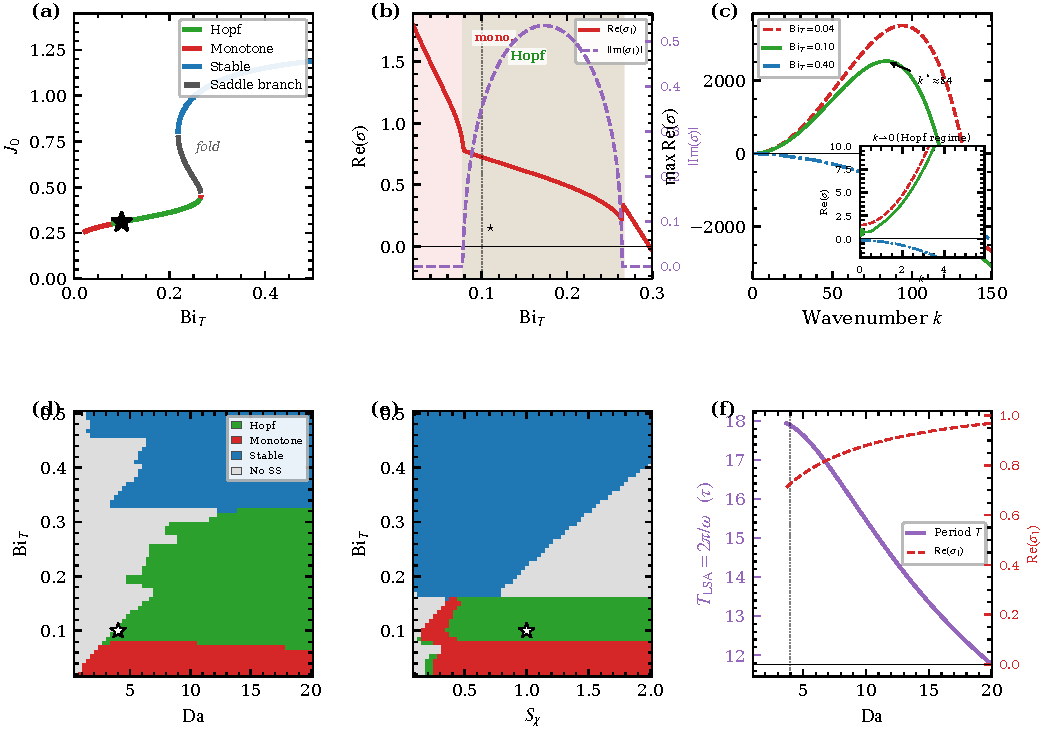
\includegraphics[width=\textwidth]{../Figure/pub/fig1_stability.pdf}
  \caption{Linear stability of the 1D slab based on the analytical
    dispersion relation. \textbf{(a)}~Steady-state branches $J_0$ versus
    $\Bi_T$, colored by the stability of the $k=0$ mode. Stable segments
    are drawn solid, unstable segments dashed, and the middle saddle
    branch is shown in gray; the star marks the working point used in
    the nonlinear simulations.
    \textbf{(b)}~Real and imaginary parts of the leading $k=0$
    eigenvalue along the collapsed branch, showing the monotone-to-Hopf
    transition and the finite $\Bi_T$ oscillation window.
    \textbf{(c)}~Dispersion curves $\max \Re(\sigma(k))$ for three
    representative $\Bi_T$ values. The inset resolves the long-wave
    behavior near $k=0$, while the main panel shows the finite-$k$
    spinodal peak.
    \textbf{(d)}~Classification map in the $(\Da,\Bi_T)$ plane:
    stable (blue), Hopf unstable (green), monotone unstable (red), and
    no admissible uniform steady state (gray).
    \textbf{(e)}~Corresponding classification map in the
    $(S_\chi,\Bi_T)$ plane.
    \textbf{(f)}~Linear period estimate $T_{\mathrm{LSA}}=2\pi/\omega$
    and growth rate $\Re(\sigma_1)$ versus $\Da$ at the working point.}
  \label{fig:stability}
\end{figure*}

\subsection{Implications for the working point}
\label{sec:0d_mechanism}

At the default parameter set used for the slab simulations, the relevant
uniform state lies on the collapsed branch in
Fig.~\ref{fig:stability}(a). Panels \textbf{(a)} and \textbf{(b)} show
that increasing $\Bi_T$ drives a sequence
monotone~$\rightarrow$~Hopf~$\rightarrow$~stable/fold: weak cooling
causes thermal runaway, intermediate cooling yields oscillatory growth,
and sufficiently strong cooling stabilizes the swollen branch or removes
the collapsed branch altogether. Panels \textbf{(d)} and \textbf{(e)}
show that this Hopf region persists only when the reaction strength
($\Da$) and LCST sensitivity ($S_\chi$) are large enough to overcome
surface heat loss.

The analytical period estimate in Fig.~\ref{fig:stability}(f),
$T_{\mathrm{LSA}}=2\pi/\omega$, provides the small-amplitude precursor
to the nonlinear oscillation period measured in the direct PDE
simulations below. Quantitative differences are expected once the orbit
reaches finite amplitude, but the dispersion analysis correctly
identifies the existence, type, and timescale of the instability that
seeds the self-oscillating slab dynamics.


%% ================================================================
%%  IV. SPATIALLY RESOLVED DYNAMICS IN THE 1D SLAB
%% ================================================================
\section{Spatially Resolved Dynamics in the 1D Slab}
\label{sec:slab}

We now turn to the full 1D slab model, which resolves spatial gradients
that are absent in the 0D reduction.

\subsection{Self-sustained oscillation mechanism}
\label{sec:osc_mech}

Figure~\ref{fig:mechanism} shows the oscillation dynamics at the default
parameters (Table~\ref{tab:params}). After a brief transient
($\sim\!3\tau$), the system settles into a limit cycle with period
$T\approx 27\tau$ and surface amplitude $\Delta J\approx 0.93$. The
oscillation follows a relaxation cycle with four distinct phases
(Fig.~\ref{fig:mechanism}(c)):
\begin{enumerate}
  \item \textbf{Swelling} ($J$ rising, $\theta\approx 0$): the gel is
    below the LCST and absorbs solvent; fresh reactant permeates the
    swollen network.
  \item \textbf{Ignition} ($\theta$ rising steeply): accumulated
    reactant drives exothermic heat release; $\theta$ crosses the LCST
    threshold.
  \item \textbf{Collapse} ($J$ dropping, $\theta$ peaked): the gel
    deswells sharply, expelling solvent and reactant; pore accessibility
    drops to near zero.
  \item \textbf{Cooling / refill} ($\theta$ falling, $J$ at minimum):
    heat dissipates through the surface while reactant access recovers;
    once $\theta<\theta_\mathrm{LCST}$, swelling restarts.
\end{enumerate}
The phase portrait (Fig.~\ref{fig:mechanism}(d)) shows a well-defined
limit cycle in the $(\langle J\rangle,\langle\theta\rangle)$ plane,
confirming the relaxation oscillator character.

\begin{figure*}[!htbp]
  \centering
  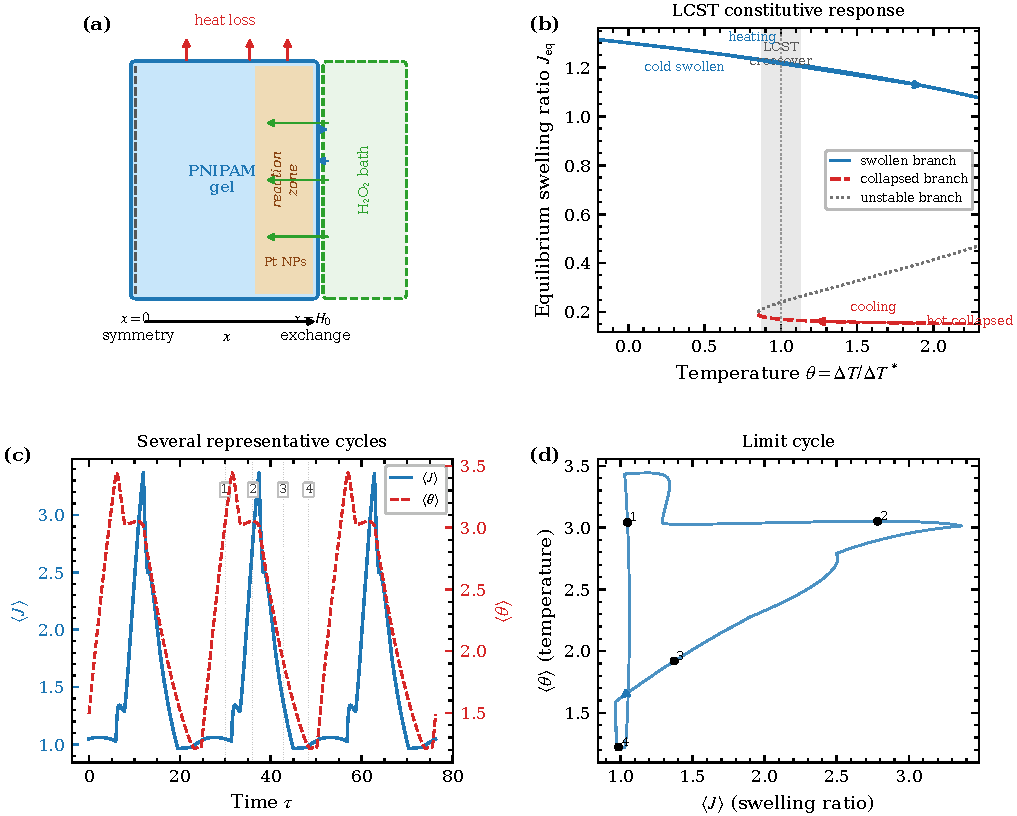
\includegraphics[width=\textwidth]{../Figure/pub/fig2_mechanism.pdf}
  \caption{Self-sustained oscillation mechanism in the 1D slab.
    \textbf{(a)}~Gel slab--bath schematic showing the three coupled
    fields and boundary conditions.
    \textbf{(b)}~Representative LCST constitutive response:
    equilibrium swelling ratio $J_\mathrm{eq}$ versus temperature
    $\theta$, showing the swollen, collapsed, and unstable branches,
    together with schematic heating and cooling trajectories across the
    LCST crossover region.
    \textbf{(c)}~Time series of $\langle J\rangle$ (blue, left axis) and
    $\langle\theta\rangle$ (red, right axis) over several representative
    cycles; numbered guides mark the four stages: swelling, ignition,
    collapse, and cooling/refill.
    \textbf{(d)}~Phase portrait showing the limit cycle in the
    $(\langle J\rangle,\langle\theta\rangle)$ plane, with numbered points
    corresponding to the four stages in panel~(c).}
  \label{fig:mechanism}
\end{figure*}

\subsection{Dual-zone termination mechanism}
\label{sec:dual_zone}

The spatial structure reveals a key feature absent from the 0D model:
the oscillation terminates through different mechanisms at different
locations. In the \emph{outer shell} ($\xi\gtrsim 0.7$), the gel
collapses sharply and the accessibility factor
$(1-\phi)^{m_\mathrm{act}}\to 0$, extinguishing the reaction even
though the local reactant concentration remains non-negligible
($u_\mathrm{surf}\approx 0.23$--$0.28$ at the collapse moment). This
is \emph{accessibility-dominated} termination: the mechanical collapse,
not reactant depletion, shuts off the heat source. After collapse,
$u_\mathrm{surf}$ rises to $\approx 1$ as the surface Robin supply
continues while the zero-accessibility shell blocks consumption; this
``stored'' reactant re-ignites the next cycle.

In the \emph{inner core} ($\xi\lesssim 0.5$), the Thiele modulus
$\Phi^2 = \Da\,(1-\phi_0)^{m_\mathrm{act}}/(\delta D_0)$ is large
enough that $u$ is depleted during the heating phase while the core
remains swollen. Here termination is \emph{reactant-depletion
dominated}. This spatial coexistence of accessibility-controlled and
depletion-controlled termination is a hallmark of the
thermo-chemo-poroelastic coupling and has no analog in spatially
uniform oscillator models.

Figure~\ref{fig:mechanismdetail} resolves this cycle directly in space
and time. The surface traces in panels \textbf{(a)}--\textbf{(c)} show
that collapse is triggered while $u_\mathrm{surf}$ remains finite,
whereas the kymographs and phase-selected profiles in
panels~\textbf{(d)}--\textbf{(g)} show that accessibility loss is
localized near the boundary and that the inner core remains reactant
limited. The mechanism is therefore genuinely dual-zone: the outer shell
is accessibility-terminated, while the interior is depletion-limited.

\begin{figure*}[!htbp]
  \centering
  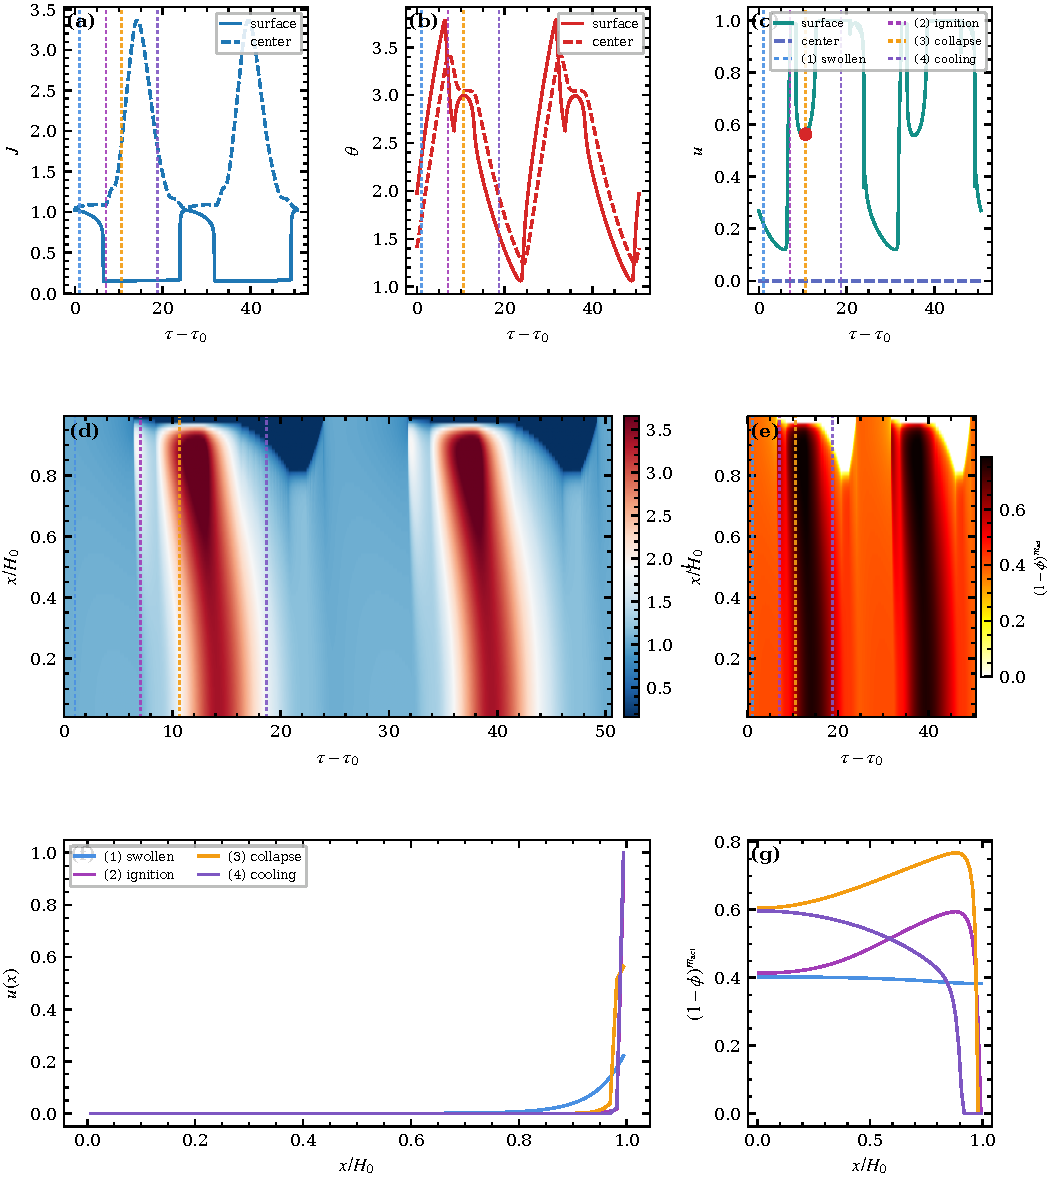
\includegraphics[width=\textwidth]{../Figure/pub/fig3_mechanism_detail.pdf}
  \caption{Detailed spatiotemporal evidence for the oscillation
    mechanism at the optimized slab parameters
    ($\Da=4$, $D_0=2$, $\Bi_c=0.70$, $\Bi_T=0.10$).
    \textbf{(a)}~Surface and center swelling-ratio traces.
    \textbf{(b)}~Surface and center temperature traces.
    \textbf{(c)}~Surface and center reactant traces; the marked collapse
    event occurs at finite $u_\mathrm{surf}$.
    \textbf{(d)}~Spatiotemporal kymograph of $J(x,\tau)$.
    \textbf{(e)}~Kymograph of the accessibility factor
    $(1-\phi)^{m_\mathrm{act}}$.
    \textbf{(f)}~Reactant profiles at the four representative phases.
    \textbf{(g)}~Accessibility profiles at the same phases.}
  \label{fig:mechanismdetail}
\end{figure*}

\subsection{Two oscillatory regimes}
\label{sec:two_regimes}

Consistent with the linear-stability predictions (Sec.~\ref{sec:0d}), the 1D slab
exhibits two qualitatively distinct oscillatory regimes
(Fig.~\ref{fig:1dslab}):

\textbf{Regime~I} ($S_\chi\lesssim 0.8$): Large-amplitude relaxation
oscillations ($\Delta J\gtrsim 0.4$) with long period ($T\gtrsim
30\tau$). Temperature excursions are large ($\Delta\theta\sim 2$--$3$),
and the spatial structure is strongly nonuniform: the surface collapses
to $J\approx 0.15$ while the center remains near equilibrium
(Fig.~\ref{fig:1dslab}(b,d,f)).

\textbf{Regime~II} ($S_\chi\gtrsim 1.0$): Small-amplitude
quasi-harmonic oscillations ($\Delta J\lesssim 0.1$, $T\lesssim
15\tau$). The gel barely crosses the LCST and the spatial profiles are
more uniform (Fig.~\ref{fig:1dslab}(a,c,e)).

The kymographs (Fig.~\ref{fig:1dslab}(c,d)) highlight the spatial
extent of the oscillation: in Regime~I, only the outer $\sim\!30\%$ of
the slab participates in the collapse--swelling cycle; in Regime~II,
the entire slab oscillates nearly uniformly.

\begin{figure*}[!htbp]
  \centering
  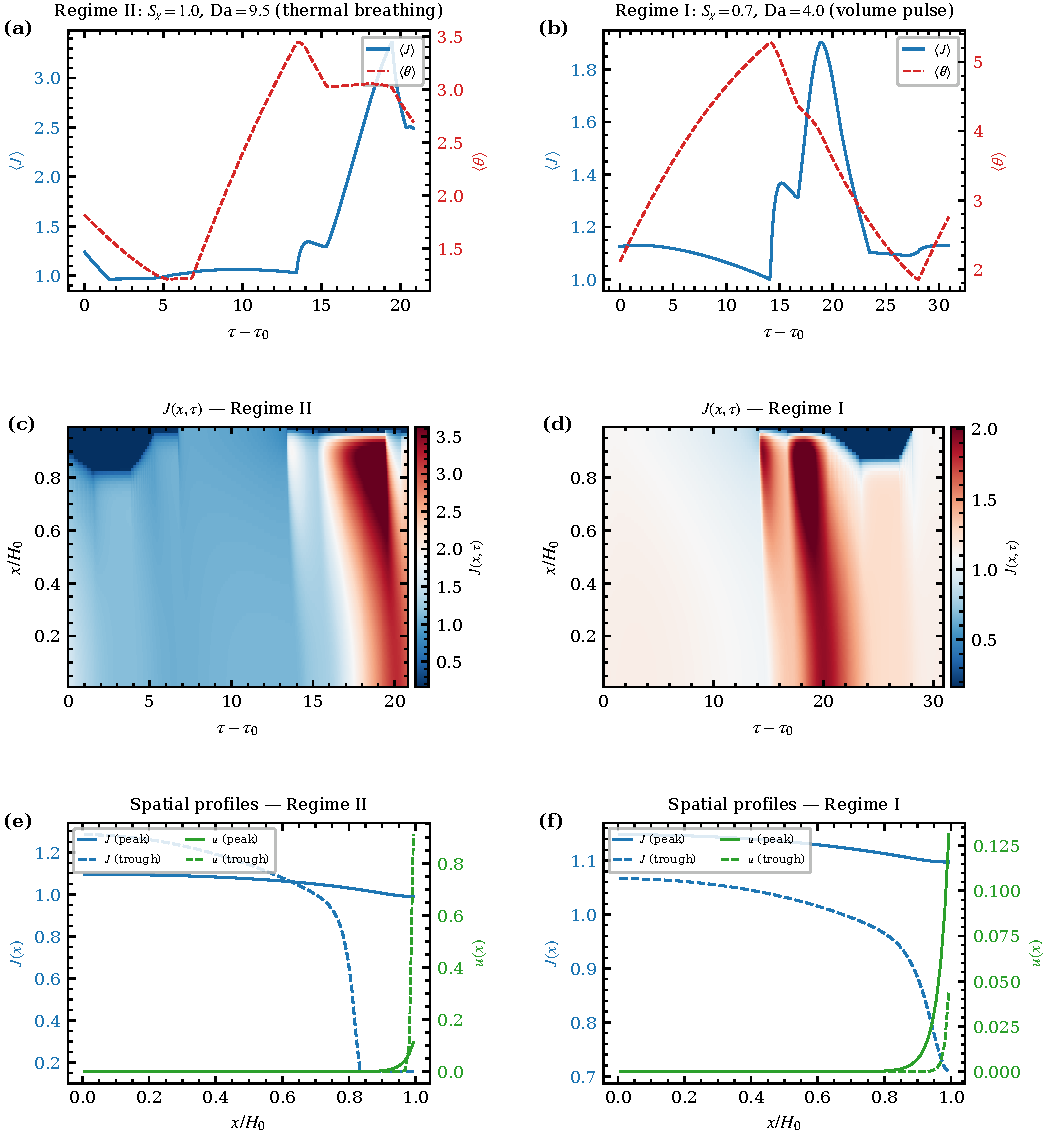
\includegraphics[width=\textwidth]{../Figure/pub/fig3_1dslab.pdf}
  \caption{Two oscillatory regimes in the 1D slab.
    \emph{Left column}: Regime~II ($\Da=9.5$, $S_\chi=1.0$);
    \emph{right column}: Regime~I ($\Da=4.0$, $S_\chi=0.7$).
    \textbf{(a,b)}~Time series of $\langle J\rangle$ (left axis) and
    $\langle\theta\rangle$ (right axis) over the last three periods.
    \textbf{(c,d)}~Kymographs of $J(\xi,t)$ showing the spatiotemporal
    structure.
    \textbf{(e,f)}~Spatial profiles of $J$ (blue), $\theta$ (red), and
    $u$ (green) at peak (solid) and trough (dashed) of the oscillation.}
  \label{fig:1dslab}
\end{figure*}

\subsection{Parameter-space phase diagram}
\label{sec:param_map}

Figure~\ref{fig:phasemap} presents the oscillation landscape in the
$(S_\chi,\Da)$ plane. The phase diagram (Fig.~\ref{fig:phasemap}(a))
distinguishes oscillatory from steady-state regions and identifies the
boundary between Regimes~I and II. The corresponding bifurcation curves
(Fig.~\ref{fig:phasemap}(b)) show that the oscillation amplitude grows
monotonically with $\Da$ in Regime~I but remains bounded in Regime~II.

The linear-stability maps in Fig.~\ref{fig:stability}(d,e) organize the
nonlinear oscillation window in the full slab simulations: oscillation
appears only inside the finite Hopf band, while low $\Bi_T$ leads to
monotone thermal runaway and large $\Bi_T$ stabilizes the swollen
branch or eliminates the collapsed uniform state altogether. The
nonlinear 1D dynamics of Fig.~\ref{fig:phasemap} therefore emerge from
this same stability structure, with quantitative shifts caused by
finite-amplitude transport delay and spatially nonuniform evolution.

The ratio $\Bi_c/\Bi_T$ governs the competition between reactant supply
and heat loss. Oscillation requires $1.5\lesssim\Bi_c/\Bi_T\lesssim 15$;
outside this window, either insufficient reactant supply or excessive
cooling prevents the thermal runaway from completing the feedback loop.
Figure~\ref{fig:phasemap}(c) shows that increasing $\Bi_c$
monotonically increases the reactant penetration depth, providing a
route to enhance interior reactant delivery.

\begin{figure*}[!htbp]
  \centering
  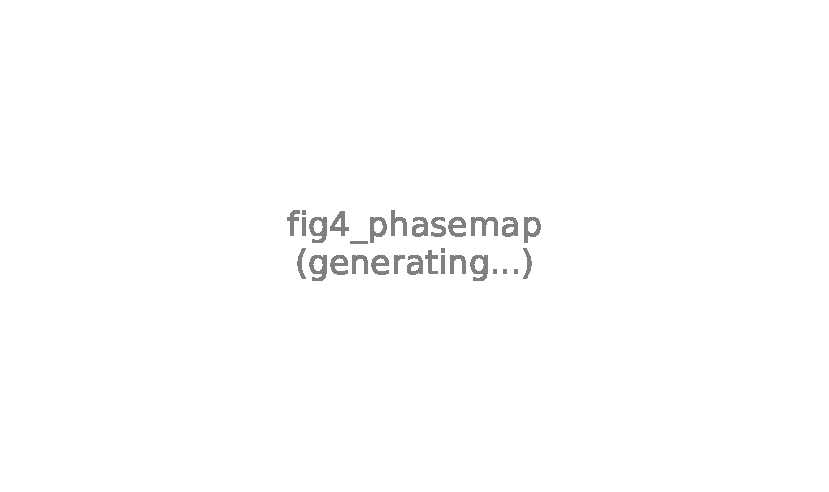
\includegraphics[width=\textwidth]{../Figure/pub/fig4_phasemap.pdf}
  \caption{Parameter-space structure of the 1D slab.
    \textbf{(a)}~$S_\chi\times\Da$ phase diagram ($16\times16$ grid,
    $N=40$, $t_\mathrm{end}=400\tau$): colors indicate oscillatory vs
    steady-state classifications; white contours show $\Delta J$ levels.
    \textbf{(b)}~Oscillation amplitude $\Delta J$ (solid) and
    $\Delta\theta$ (dashed) vs $\Da$ for Regime~I ($S_\chi=0.7$, red)
    and Regime~II ($S_\chi=1.0$, blue).
    \textbf{(c)}~Reactant penetration depth $\ell_u/H_0$ vs $\Bi_c$ at
    $\Da=9.5$, $S_\chi=1.0$.}
  \label{fig:phasemap}
\end{figure*}


%% ================================================================
%%  V. GEOMETRY EFFECTS: SLAB VS SPHERE
%% ================================================================
\section{Geometry Effects: Slab vs.\ Sphere}
\label{sec:geometry}

The instability and oscillation mechanism identified in
Secs.~\ref{sec:0d}--\ref{sec:slab} relies on the interplay between
surface-driven heat loss, reactant supply, and the gel's
volume-collapse response. Geometry affects each of these processes
through the surface-to-volume ratio and the form of the divergence
operator. We now compare the 1D slab with the 1D spherically symmetric
geometry.

\subsection{Isotropic sphere model}

We first consider a spherical gel bead with the same material parameters
as the slab but with the isotropic elastic energy $\mu_\mathrm{el}=
\Omega_e(J^{-1/3}-J^{-1})$, neglecting the distinction between radial
and circumferential stretches. The governing equations are identical to
Eqs.~\eqref{eq:governing} except that the spatial operators acquire the
spherical factor $(1/s^2)\partial_s(s^2\cdot)$.

\subsection{Critical diffusion coupling}

To probe the effect of internal transport, we introduce a diffusion
coupling parameter $\varepsilon_\mathrm{diff}$ that continuously
interpolates between a surface-only model ($\varepsilon_\mathrm{diff}
=0$, where only the outermost shell exchanges with the bath) and the
fully coupled model ($\varepsilon_\mathrm{diff}=1$).
Figure~\ref{fig:geometry}(b) shows the oscillation amplitude
$\Delta\theta$ as a function of $\varepsilon_\mathrm{diff}$:
\begin{itemize}
  \item At $\varepsilon_\mathrm{diff}=0$, the sphere oscillates with
    dynamics qualitatively similar to the slab
    (Fig.~\ref{fig:geometry}(d)).
  \item Above a critical threshold $\varepsilon^*\approx 3\times
    10^{-4}$, the oscillation amplitude drops to zero and the system
    settles into a steady swollen state
    (Fig.~\ref{fig:geometry}(e)).
\end{itemize}

The oscillation-killing mechanism is geometric: in the sphere, the
surface-to-volume ratio $3/R$ is larger than the slab's $1/H_0$, and
solvent can permeate the gel from all directions. The enhanced radial
influx creates an expanding swelling wavefront that outpaces the
collapse domain. Once the wavefront reaches the center, the entire gel
is swollen before the thermal runaway can complete, and the oscillation
dies.

\subsection{Anisotropic stress effects}

In a spherical geometry, radial and circumferential stretches differ
($\lambda_r\neq\lambda_\theta$), generating anisotropic stress. The
full-mechanics model reconstructs the current radius
$r^3(R)=3\int_0^R J\,R'^2\,dR'$, computes $\lambda_r=J/\lambda_\theta^2$,
and solves the stress equilibrium $\partial\sigma_r/\partial r +
(2/r)(\sigma_r-\sigma_\theta)=0$ to obtain a nonlocal radial stress
correction $\Sigma_r(R)$ that enters the chemical potential.

This stress locking creates a core--shell quasi-equilibrium: the
interior remains at $J\approx 0.7$, and the anisotropic stress
prevents the radial relaxation needed to complete the
swelling--collapse cycle. As a result, the full-mechanics sphere does
not oscillate at normal diffusion coupling, even in parameter regimes
where the slab and 0D models predict robust oscillation.

\subsection{Physical implications}

The geometry comparison reveals that the slab is the most favorable
geometry for thermal oscillation:
\begin{itemize}
  \item \textbf{Slab}: single exposed surface $\to$ limited solvent
    influx $\to$ collapse is effective $\to$ oscillation is robust.
  \item \textbf{Sphere}: all-round exposure $\to$ rapid radial influx
    $\to$ swelling wavefront escapes collapse domain $\to$ oscillation
    suppressed.
\end{itemize}
This finding provides direct guidance for experimental design: flat
membranes or thin films should be preferred over spherical beads for
realizing thermally driven gel oscillators.

\begin{figure*}[!htbp]
  \centering
  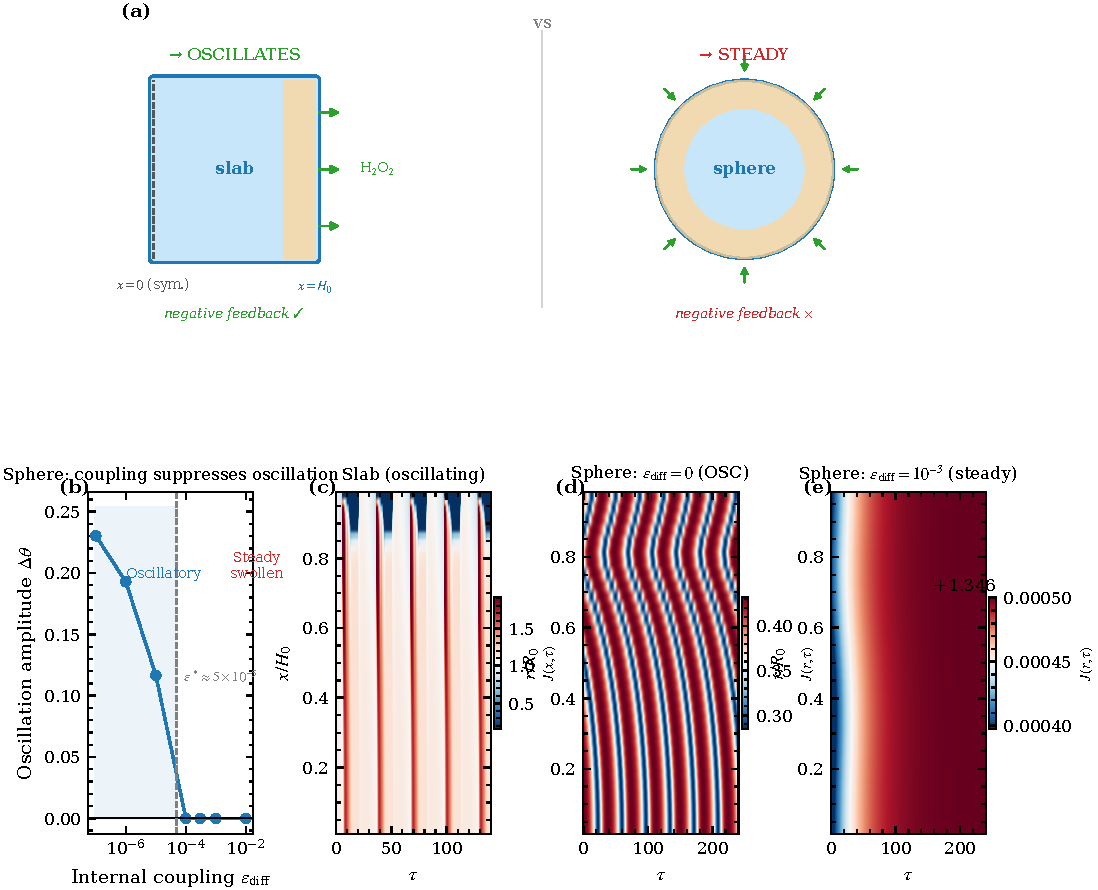
\includegraphics[width=\textwidth]{../Figure/pub/fig5_geometry.pdf}
  \caption{Geometry effects on oscillation.
    \textbf{(a)}~Schematics of slab (left) and sphere (right)
    geometries with boundary conditions.
    \textbf{(b)}~Oscillation amplitude $\Delta\theta$ vs diffusion
    coupling $\varepsilon_\mathrm{diff}$ in the sphere; the critical
    threshold $\varepsilon^*\approx 3\times 10^{-4}$ is marked.
    \textbf{(c)}~Slab kymograph $J(\xi,t)$ at Regime~I parameters
    (reference case, oscillates).
    \textbf{(d)}~Sphere kymograph at $\varepsilon_\mathrm{diff}=0$
    (surface-only model, oscillates).
    \textbf{(e)}~Sphere kymograph at $\varepsilon_\mathrm{diff}=10^{-3}$
    (fully coupled, steady state).}
  \label{fig:geometry}
\end{figure*}


%% ================================================================
%%  VI. REACTANT PENETRATION ENHANCEMENT
%% ================================================================
\section{Reactant Penetration Enhancement}
\label{sec:penetration}

For applications such as periodic chemical delivery or pulsatile drug
release, it is essential that the reactant penetrate deep into the gel
interior. We now characterize the penetration depth and identify
optimization strategies.

\subsection{Accessibility gradient and dual-regime structure}

The interior reactant concentration depends on the competition between
diffusion supply and reaction consumption, quantified by the Thiele
modulus $\Phi^2=\Da\,(1-\phi_0)^{m_\mathrm{act}}/(\delta D_0)$.
Figure~\ref{fig:penetration}(a) shows the center reactant concentration
$u_\mathrm{ctr}$ as a function of $\Da$: at high $\Da$, the interior
is completely depleted ($u_\mathrm{ctr}\to 0$), while at low $\Da$,
significant reactant persists throughout the cycle.

The accessibility front depth $x^*$---the fractional depth at which
$u>0.05$ at collapse onset---follows the Thiele scaling
(Fig.~\ref{fig:penetration}(b)):
\begin{equation}
  x^*\sim\Phi^{-1} = \sqrt{\frac{\delta D_0}{\Da\cdot
  \overline{\alpha}_\mathrm{h}\cdot\overline{f}_\mathrm{h}}},
\end{equation}
where $\overline{\alpha}_\mathrm{h}$ and $\overline{f}_\mathrm{h}$ are
the accessibility and Arrhenius factors at mid-heating conditions.

\subsection{Da--$\Gamma_A$ mechanism map}

Figure~\ref{fig:penetration}(c) maps the oscillation mechanism in the
$(\Da,\Gamma_A)$ plane. Two regimes emerge:
\begin{enumerate}
  \item \textbf{Depletion-dominated} (large $\Da$, small $\Gamma_A$):
    the inner core is starved of reactant; termination occurs by
    depletion in the interior and accessibility collapse at the surface.
  \item \textbf{Accessibility-dominated} (small $\Da$, large
    $\Gamma_A$): reactant persists throughout the gel; termination
    everywhere occurs via the pore-closure mechanism.
\end{enumerate}
The boundary satisfies
\begin{equation}
  \Da^* = \frac{\delta D_0}{(1-\phi_0/J_\mathrm{ctr})^{m_\mathrm{act}}
  \exp\!\bigl(\Gamma_A\theta_h/(1+\theta_h)\bigr)},
\end{equation}
evaluated at $\theta_h\approx 1.5$ and $J_\mathrm{ctr}\approx 1.15$.

\subsection{Optimization strategy}

We identify a three-parameter strategy to maximize interior penetration
while maintaining oscillation:
\begin{enumerate}
  \item \textbf{Reduce $\Da$}: slower reaction allows diffusion to
    carry $u$ deeper. Reducing from $\Da=14$ to $\Da=4$ increases
    $u_\mathrm{mid}$ by $\sim\!100\times$.
  \item \textbf{Increase $D_0$}: higher diffusivity accelerates
    interior supply. $D_0=2$ gives full penetration, but $D_0>2.5$
    homogenizes $u$ and destroys the spatial feedback needed for
    oscillation.
  \item \textbf{Increase $\Bi_c$}: stronger surface supply compensates
    for the lower $\Da$.
\end{enumerate}

At the optimized parameters ($\Da=4$, $D_0=2$, $\Bi_c=0.70$,
$\Bi_T=0.10$), the mid-slab reactant concentration reaches
$u_\mathrm{mid}^\mathrm{peak}=4.5\times 10^{-3}$---a
$\mathbf{590\times}$ enhancement over the original parameter set
($\Da=14$, $D_0=1$, $\Bi_c=0.35$: $u_\mathrm{mid}^\mathrm{peak}
\approx 7.6\times 10^{-6}$)---while preserving $\Delta J\approx 0.93$
and achieving full-domain penetration
(Fig.~\ref{fig:optimizationcompare}).

\begin{figure*}[!htbp]
  \centering
  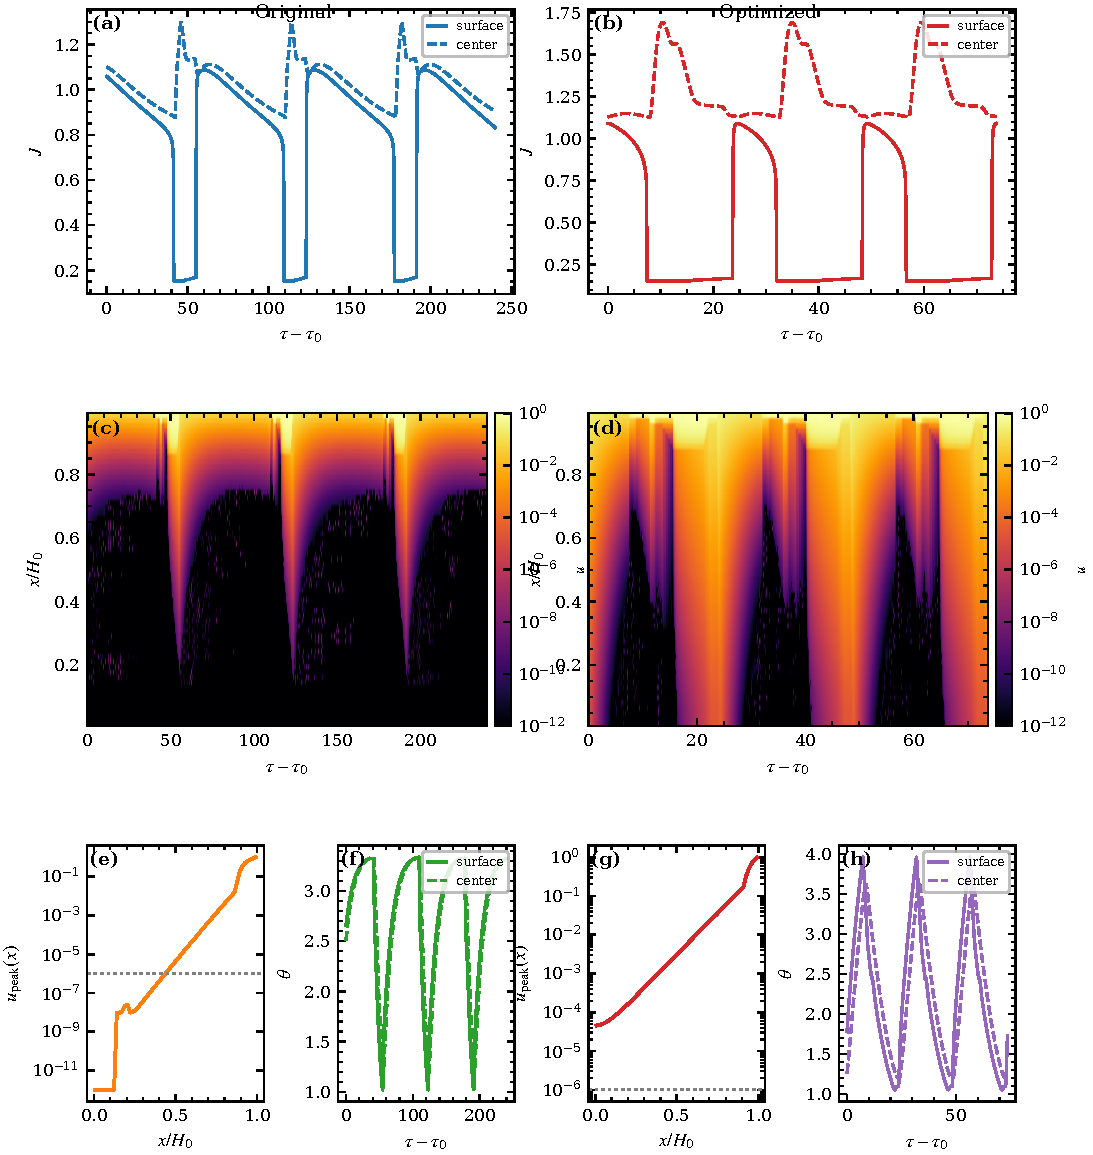
\includegraphics[width=\textwidth]{../Figure/pub/fig7_optimization_compare.pdf}
  \caption{Original-versus-optimized penetration dynamics.
    Left column pair: original parameters
    ($\Da=14$, $D_0=1$, $\Bi_c=0.35$).
    Right column pair: optimized parameters
    ($\Da=4$, $D_0=2$, $\Bi_c=0.70$).
    \textbf{(a,b)}~Surface and center swelling-ratio traces.
    \textbf{(c,d)}~Reactant kymographs $u(x,\tau)$.
    \textbf{(e,g)}~Peak reactant profiles $u_\mathrm{peak}(x)$, showing
    the large increase in interior penetration after optimization.
    \textbf{(f,h)}~Surface and center temperature traces, confirming that
    the optimized state remains oscillatory while substantially improving
    interior reactant delivery.}
  \label{fig:optimizationcompare}
\end{figure*}

\begin{figure*}[!htbp]
  \centering
  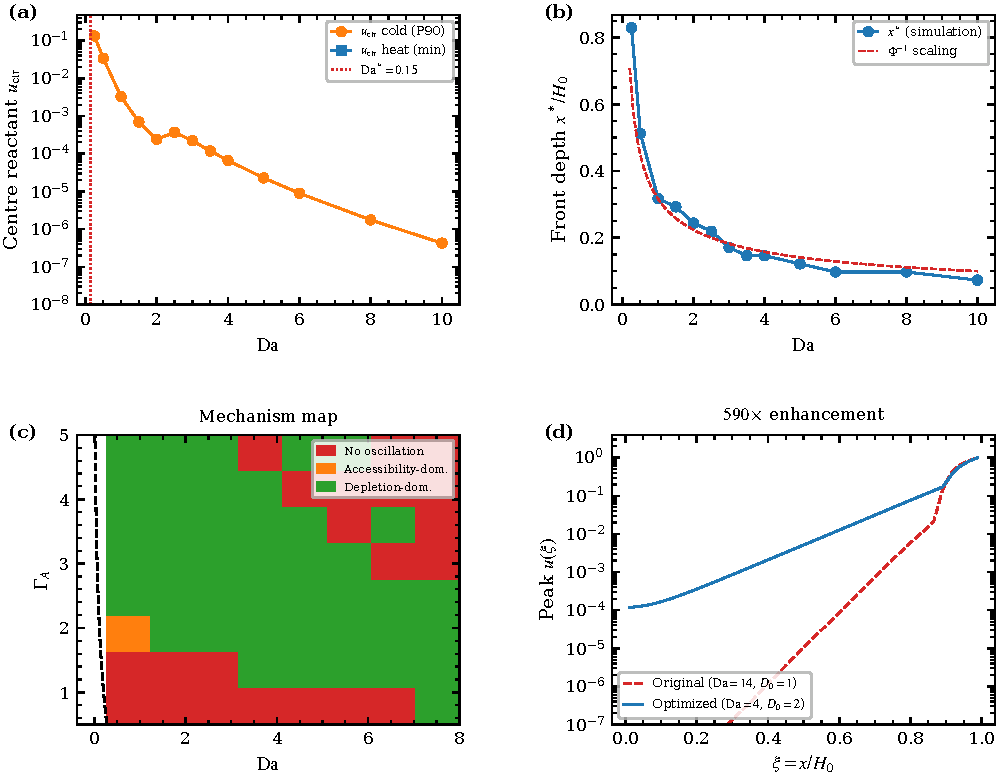
\includegraphics[width=\textwidth]{../Figure/pub/fig6_penetration.pdf}
  \caption{Reactant penetration analysis and optimization.
    \textbf{(a)}~Centre reactant $u_\mathrm{ctr}$ vs $\Da$: cold-phase
    value (orange, 90th percentile) and heating-phase minimum (blue);
    red dotted line marks analytical $\Da^*$.
    \textbf{(b)}~Accessibility front depth $x^*$ vs $\Da$ (circles),
    with analytical $\Phi^{-1}$ scaling (red dashed).
    \textbf{(c)}~$\Da\times\Gamma_A$ mechanism map: yellow =
    accessibility-dominated, green = depletion-dominated, red = no
    oscillation; dashed curve = analytical $\Da^*(\Gamma_A)$ boundary.
    \textbf{(d)}~Spatial profiles of $u(\xi)$ comparing the original
    ($\Da=14$, $D_0=1$) and optimized ($\Da=4$, $D_0=2$) parameters,
    demonstrating $590\times$ enhancement of interior reactant level.}
  \label{fig:penetration}
\end{figure*}


%% ================================================================
%%  VII. DISCUSSION
%% ================================================================
\section{Discussion}
\label{sec:discussion}

\subsection{Model hierarchy: 0D to 1D validation}

The 0D lumped model successfully predicts the Hopf bifurcation boundaries
and the existence of two oscillatory regimes, validating its use as a
rapid screening tool for parameter exploration. The 1D slab confirms
these predictions while adding crucial spatial physics: the dual-zone
termination mechanism, nonuniform oscillation profiles, and the
surface-reactant storage effect. Quantitatively, the 0D and 1D critical
$\Da$ values agree to within $\sim\!20\%$, with discrepancies
attributable to the transport delay introduced by finite diffusion
lengths.

\subsection{Geometry selection for experiments}

Our geometry comparison provides clear experimental guidance: flat
membranes or thin films are strongly preferred over spherical beads for
realizing thermally driven oscillators. The sphere's enhanced
surface-to-volume ratio and anisotropic stress effects conspire to
suppress the collapse--swelling cycle. This finding may explain why
Siegel's original spherical-bead experiments~\cite{Siegel1988} required
carefully tuned conditions, while slab-geometry
demonstrations~\cite{Zarzycki2020} were more robust.

\subsection{Application to chemical delivery}

The dual-zone termination mechanism has implications for autonomous
chemical delivery. The ``stored reactant'' phase
($u_\mathrm{surf}\approx 1$ during the collapsed state) provides a
built-in reservoir that ensures reliable re-ignition, making the
oscillation self-sustaining. The $590\times$ penetration enhancement
demonstrates that the pulsatile pumping mechanism can deliver reactant
deep into the gel interior, provided the $\Da$--$D_0$--$\Bi_c$
combination is properly tuned. The counter-intuitive role of the
accessibility exponent $m_\mathrm{act}$ deserves emphasis: higher
$m_\mathrm{act}$ (sharper pore blockage) increases $u_\mathrm{mid}$
because it amplifies the $J$ oscillation, driving stronger pulsatile
injection during the swelling phase.

\subsection{Limitations}

The present model is one-dimensional and assumes uniaxial (slab) or
isotropic (sphere) swelling; in three dimensions, shape changes and
lateral stress could couple to the oscillation frequency. We neglect
convective heat transfer ($\Pe_T=0$) and mechanically mediated reactant
transport. These are small corrections at the parameters studied
(Appendix~\ref{app:numerics}). The model also assumes a single
irreversible reaction; multi-step kinetics (as in the BZ reaction) may
introduce additional dynamic complexity including period-doubling and
chaos, which we leave to future work.


%% ================================================================
%%  VIII. CONCLUSION
%% ================================================================
\section{Conclusion}
\label{sec:conclusion}

We have developed and analyzed a hierarchy of models---from analytical
linear stability to spatially resolved 1D slab and sphere dynamics---for self-oscillating
thermoresponsive gels driven by an exothermic reaction. The key
contributions are:
\begin{enumerate}
  \item A \emph{systematic dimensionless framework} reducing the
    parameter space to eight groups with clear physical interpretations,
    enabling efficient exploration of the oscillation landscape.
  \item \emph{0D Hopf bifurcation analysis} identifying the critical
    conditions for oscillation onset in the $(\Da,S_\chi)$ plane and
    predicting two oscillatory regimes: a large-amplitude relaxation
    oscillator (Regime~I) and a small-amplitude quasi-harmonic oscillator
    (Regime~II).
  \item \emph{Spatially resolved 1D slab dynamics} revealing the
    four-phase relaxation cycle, the dual-zone termination mechanism
    (accessibility-dominated outer shell vs.\ depletion-dominated inner
    core), and surface reactant storage enabling reliable re-ignition.
  \item \emph{Geometry-dependent oscillation}: the slab sustains robust
    oscillations, whereas the sphere suppresses them due to enhanced
    radial solvent influx and anisotropic stress locking. The critical
    diffusion coupling threshold is $\varepsilon^*\approx 3\times
    10^{-4}$.
  \item \emph{Reactant penetration optimization}: a $590\times$
    enhancement of interior reactant concentration is achieved by
    simultaneously reducing $\Da$ and increasing $D_0$ and $\Bi_c$,
    while maintaining oscillation. The Thiele-modulus scaling provides
    a predictive design rule.
\end{enumerate}

Future work will extend the model to two and three dimensions, map the
full bifurcation diagram including period-doubling routes, and compare
quantitatively with experimental observations on PNIPAM systems coupled
to exothermic reactions.

\begin{acknowledgments}
[Acknowledgments placeholder.]
\end{acknowledgments}

\begin{thebibliography}{99}
\bibitem{Yoshida2010} R.~Yoshida and T.~Ueki, NPG Asia Mater.\ \textbf{6}, e107 (2014).
\bibitem{Yoshida2002} R.~Yoshida, T.~Takahashi, T.~Yamaguchi, and H.~Ichijo, J.~Am.\ Chem.\ Soc.\ \textbf{118}, 5134 (1996).
\bibitem{Yoshida2004} R.~Yoshida, Adv.\ Mater.\ \textbf{22}, 3463 (2010).
\bibitem{Yashin2006} V.~V.~Yashin and A.~C.~Balazs, Science \textbf{314}, 798 (2006).
\bibitem{Siegel1988} R.~A.~Siegel and B.~A.~Firestone, Macromolecules \textbf{21}, 3254 (1988).
\bibitem{Siegel1992} R.~A.~Siegel, Adv.\ Polym.\ Sci.\ \textbf{109}, 233 (1993).
\bibitem{Zarzycki2020} R.~Zarzycki, J.\ Controlled Release \textbf{317}, 1 (2020).
\bibitem{Boissonade2003} J.~Boissonade, Phys.\ Rev.\ Lett.\ \textbf{90}, 188302 (2003).
\bibitem{Flory1953} P.~J.~Flory, \textit{Principles of Polymer Chemistry} (Cornell University Press, Ithaca, 1953).
\bibitem{Tanaka1979} T.~Tanaka, Phys.\ Rev.\ Lett.\ \textbf{40}, 820 (1978).
\bibitem{TanakaFillmore1979} T.~Tanaka and D.~J.~Fillmore, J.\ Chem.\ Phys.\ \textbf{70}, 1214 (1979).
\bibitem{Heskins1968} M.~Heskins and J.~E.~Guillet, J.\ Macromol.\ Sci.\ A \textbf{2}, 1441 (1968).
\bibitem{Hirotsu1987} S.~Hirotsu, Y.~Hirokawa, and T.~Tanaka, J.\ Chem.\ Phys.\ \textbf{87}, 1392 (1987).
\bibitem{Schild1992} H.~G.~Schild, Prog.\ Polym.\ Sci.\ \textbf{17}, 163 (1992).
\bibitem{Shibayama1993} M.~Shibayama and T.~Tanaka, Adv.\ Polym.\ Sci.\ \textbf{109}, 1 (1993).
\bibitem{Quesada2011} M.~Quesada-P\'erez, J.~A.~Maroto-Centeno, J.~Forcada, and R.~Hidalgo-Alvarez, Soft Matter \textbf{7}, 10536 (2011).
\bibitem{Doi2009} M.~Doi, J.\ Phys.\ Soc.\ Jpn.\ \textbf{78}, 052001 (2009).
\bibitem{Hong2008} W.~Hong, X.~Zhao, J.~Zhou, and Z.~Suo, J.\ Mech.\ Phys.\ Solids \textbf{56}, 1779 (2008).
\bibitem{Chester2010} S.~A.~Chester and L.~Anand, J.\ Mech.\ Phys.\ Solids \textbf{58}, 1879 (2010).
\bibitem{Lucantonio2013} A.~Lucantonio, P.~Nardinocchi, and L.~Teresi, J.\ Mech.\ Phys.\ Solids \textbf{61}, 205 (2013).
\bibitem{Kuksenok2014} O.~Kuksenok and A.~C.~Balazs, Adv.\ Funct.\ Mater.\ \textbf{23}, 4601 (2013).
\bibitem{Dayal2012} P.~Dayal, O.~Kuksenok, and A.~C.~Balazs, Soft Matter \textbf{8}, 3814 (2012).
\bibitem{Turing1952} A.~M.~Turing, Philos.\ Trans.\ R.\ Soc.\ B \textbf{237}, 37 (1952).
\bibitem{Karg2008} M.~Karg, I.~Pastoriza-Santos, L.~M.~Liz-Marz\'an, and T.~Hellweg, ChemPhysChem \textbf{7}, 2298 (2006).
\end{thebibliography}

\appendix

%% ================================================================
%%  Appendix A: Model Construction
%% ================================================================
\section{Model Construction}
\label{app:model}

We formulate a one-dimensional Lagrangian model for the coupled thermo-chemo-poroelastic dynamics of a thermoresponsive gel slab undergoing an exothermic reaction. The primary variables are the local swelling ratio $J(X,t)$, reactant concentration $c(X,t)$, and temperature $T(X,t)$.

\subsection{Kinematics}

Consider a gel slab of reference (dry-state) thickness $H_0$. We adopt a material (Lagrangian) coordinate $X\in[0,H_0]$, with $X=0$ denoting the symmetry plane and $X=H_0$ the free surface. The current position of a material point is $x(X,t)$, and the local volume ratio is
\begin{equation}
  J(X,t) = \frac{\partial x}{\partial X} > 0.
  \label{eq:J_def}
\end{equation}
In one dimension, $J$ is the local swelling ratio. The polymer volume fraction is a dependent variable determined by mass conservation of the network:
\begin{equation}
  \phi(X,t) = \frac{\pp}{J(X,t)},
  \label{eq:phi_J}
\end{equation}
where $\pp$ is the polymer volume fraction in the reference state. The current thickness of the slab is
\begin{equation}
  h(t) = x(H_0,t) = \int_0^{H_0} J(X,t)\,dX.
  \label{eq:thickness}
\end{equation}

\subsection{Governing equations}

\subsubsection{Swelling--permeation equation}

The evolution of $J$ is governed by solvent conservation:
\begin{equation}
  \frac{\partial J}{\partial t} = -\frac{\partial Q_s}{\partial X},
  \label{eq:J_evol}
\end{equation}
where $Q_s$ is the solvent flux relative to the polymer network, driven by chemical-potential gradients:
\begin{equation}
  Q_s = -M_s(J,T)\,\frac{\partial \mu_s}{\partial X}.
  \label{eq:Qs}
\end{equation}
Here $M_s(J,T)$ is the permeation mobility and $\mu_s$ is the solvent chemical potential.

\subsubsection{Reactant transport equation}

The reactant concentration $c(X,t)$ (moles per current volume of pore fluid) evolves according to
\begin{equation}
  \frac{\partial (Jc)}{\partial t}
  + \frac{\partial N_c}{\partial X}
  = -J\,R(c,T,J),
  \label{eq:c_evol}
\end{equation}
with the total reactant flux
\begin{equation}
  N_c = c\,Q_s - D_c(J,T)\,\frac{\partial c}{\partial X}.
  \label{eq:Nc}
\end{equation}
The first term represents advective transport by the solvent flow, and the second term Fickian diffusion within the pore fluid. The effective diffusivity $D_c(J,T)$ depends on the local microstructure via $J$.

\subsubsection{Heat equation}

The temperature field satisfies
\begin{equation}
  C_\mathrm{eff}(J)\,\frac{\partial T}{\partial t}
  = \frac{\partial}{\partial X}\!\left(K_T(J)\,\frac{\partial T}{\partial X}\right)
  - \frac{\partial}{\partial X}\!\left(c_p^\ell\,T\,Q_s\right)
  + (-\Delta H_r)\,J\,R(c,T,J),
  \label{eq:T_evol}
\end{equation}
where $C_\mathrm{eff}(J)$ is the effective volumetric heat capacity, $K_T(J)$ is the effective thermal conductivity, $c_p^\ell$ is the solvent heat capacity per unit volume, and $-\Delta H_r > 0$ is the exothermic reaction enthalpy. The three terms on the right-hand side represent, respectively, thermal conduction, enthalpy advection by the solvent flow, and reaction heat generation.

\subsection{Free energy and chemical potential}

The Helmholtz free-energy density per unit reference volume is written as
\begin{equation}
  \Psi(J,T) = \Psi_\mathrm{el}(J) + \Psi_\mathrm{mix}(\phi,T)
  + \frac{\kappa_J}{2}\left(\frac{\partial J}{\partial X}\right)^2,
  \label{eq:Psi}
\end{equation}
where $\phi = \pp/J$, and the three contributions are the elastic energy of the network, the Flory--Huggins mixing energy, and a gradient-energy regularization.

The mixing free-energy density takes the standard Flory--Huggins form:
\begin{equation}
  \Psi_\mathrm{mix}(\phi,T)
  = \frac{R_g T}{v_s}
  \Big[(1-\phi)\ln(1-\phi) + \chi(T,\phi)\,\phi(1-\phi)\Big],
  \label{eq:Psi_mix}
\end{equation}
with $R_g$ the gas constant, $v_s$ the solvent molar volume, and the Flory--Huggins interaction parameter
\begin{equation}
  \chi(T,\phi) = \chi_0(T) + \chi_1\,\phi.
  \label{eq:chi}
\end{equation}
The temperature-dependent part $\chi_0(T)$ encodes the lower critical solution temperature (LCST) behavior of the gel.

The solvent chemical potential is then
\begin{equation}
  \mu_s = \mu_\mathrm{mix}(J,T) + \mu_\mathrm{el}(J)
  - \kappa_J\,\frac{\partial^2 J}{\partial X^2},
  \label{eq:mu_s}
\end{equation}
or equivalently a generalized swelling stress:
\begin{equation}
  \Sigma(J,T) = \Sigma_\mathrm{el}(J) - \Sigma_\mathrm{mix}(J,T)
  - \kappa_J\,\frac{\partial^2 J}{\partial X^2},
  \label{eq:Sigma}
\end{equation}
with the solvent flux alternatively expressed as $Q_s = -M_s(J,T)\,\partial_X \Sigma$.

\subsection{Reaction kinetics}

The volumetric reaction rate takes the Arrhenius form modulated by a collapse-dependent accessibility factor:
\begin{equation}
  R(c,T,J) = k_0\,c^n\,\exp\!\left(-\frac{E_a}{R_g T}\right) a(J),
  \label{eq:R}
\end{equation}
where $k_0$ is the pre-exponential factor, $n$ the reaction order, and $E_a$ the activation energy.

The activity factor $a(J)$ models the suppression of reaction due to reduced free solvent volume upon collapse:
\begin{equation}
  a(J) = \left(1 - \frac{\pp}{J}\right)^m = (1-\phi)^m.
  \label{eq:aJ}
\end{equation}
When the gel collapses ($J\to\pp$, $\phi\to 1$), the activity vanishes, shutting off the reaction.

The effective transport coefficients similarly depend on the microstructure:
\begin{align}
  D_c(J) &= D_0\left(1-\frac{\pp}{J}\right)^{m_D}, \label{eq:Dc} \\
  M_s(J) &= M_0\left(1-\frac{\pp}{J}\right)^{m_M}, \label{eq:Ms}
\end{align}
so that both solute diffusion and solvent permeation are suppressed in the collapsed state.

\subsection{Oscillation mechanism}

The coupled model gives rise to a closed feedback loop:
\begin{enumerate}
  \item Reactant enters through the surface and is consumed, releasing heat.
  \item Temperature rises, increasing $\chi$ and driving the gel toward collapse ($J\downarrow$).
  \item Collapse reduces pore size, suppressing both permeation ($M_s\downarrow$) and diffusion ($D_c\downarrow$), as well as reaction accessibility ($a=(1-\phi)^{m_\mathrm{act}}\downarrow$).
  \item The heat source is extinguished; the gel cools by conduction and surface exchange.
  \item Cooling lowers $\chi$; the gel re-swells ($J\uparrow$), reopening transport pathways.
  \item Fresh reactant enters, and the cycle repeats.
\end{enumerate}
Self-sustained oscillation requires sufficient time-scale separation between the fast positive feedback (reaction $\to$ heating $\to$ collapse) and the slow negative feedback (collapse $\to$ transport suppression $\to$ cooling $\to$ re-swelling).

The reaction shutoff in step~3 is spatially heterogeneous. In the outer
shell ($\xi\gtrsim 0.7$), the collapse drives $a\to 0$ while the local
reactant concentration is still finite ($u_\mathrm{surf}\approx 0.25$);
shutoff is \emph{accessibility-controlled}. In the inner core
($\xi\lesssim 0.5$), the Thiele modulus is large enough that $u$ depletes
before the core collapses; shutoff there is \emph{reactant-depletion
controlled}. Post-collapse, the surface Robin supply refills $u_\mathrm{surf}$
to $\approx 1$ (the collapsed shell blocks consumption), ``storing'' reactant
for the next re-ignition.

\subsection{Boundary conditions}

At the symmetry plane $X=0$:
\begin{equation}
  Q_s = 0, \qquad N_c = 0, \qquad \frac{\partial T}{\partial X} = 0.
  \label{eq:bc_sym}
\end{equation}

At the free surface $X=H_0$:

\paragraph{Solvent exchange.}
A Robin-type condition couples the surface chemical potential to the bath:
\begin{equation}
  Q_s = L_\mu\!\left(\mu_s - \mu_\mathrm{bath}\right),
  \label{eq:bc_mu}
\end{equation}
where $L_\mu$ is a surface transfer coefficient. In the limit of rapid equilibration, $\mu_s = \mu_\mathrm{bath}$.

\paragraph{Reactant supply.}
\begin{equation}
  N_c = k_c\,(c - c_b),
  \label{eq:bc_c}
\end{equation}
where $c_b$ is the constant bath concentration.

\paragraph{Heat exchange.}
\begin{equation}
  -K_T\,\frac{\partial T}{\partial X} = h_T\,(T - T_\infty),
  \label{eq:bc_T}
\end{equation}
where $h_T$ is the surface heat-transfer coefficient and $T_\infty$ the ambient temperature.

\paragraph{Mechanical boundary.}
The free surface is traction-free. In the $J$-formulation this is implicitly satisfied by the chemical-potential balance.

%% ================================================================
%%  Appendix B: Nondimensionalization
%% ================================================================
\section{Nondimensionalization}
\label{app:nondim}

\subsection{Scaling}

We introduce the following dimensionless variables. Length is scaled by the reference thickness:
\begin{equation}
  X = H_0\,\tilde{x}, \qquad \tilde{x}\in[0,1].
\end{equation}
The swelling ratio $J$ is already dimensionless. Reactant concentration is normalized by the bath value:
\begin{equation}
  c = c_b\,u.
\end{equation}
Temperature is measured relative to ambient, scaled by the adiabatic reaction temperature rise:
\begin{equation}
  T = T_\infty + \Delta T_*\,\theta,
  \qquad
  \Delta T_* = \frac{(-\Delta H_r)\,c_b}{C_*},
\end{equation}
where $C_*$ is a representative volumetric heat capacity.

The chemical potential is scaled by the thermal mixing energy:
\begin{equation}
  \mu_s = \mu_*\,m, \qquad \mu_* = \frac{R_g T_\infty}{v_s}.
\end{equation}

Time is scaled by the swelling/permeation time:
\begin{equation}
  \tau_s = \frac{H_0^2}{M_0\,\mu_*},
\end{equation}
where $M_0$ is a reference mobility. The solvent and reactant flux scales follow:
\begin{equation}
  Q_s = \frac{H_0}{\tau_s}\,q,
  \qquad
  N_c = \frac{c_b\,H_0}{\tau_s}\,n.
\end{equation}

Material functions are factored as reference value times dimensionless function:
\begin{align}
  M_s &= M_0\,\Ms(J,\theta), &
  D_c &= D_0\,\Ds(J,\theta), \\
  C_\mathrm{eff} &= C_*\,\Cs(J), &
  K_T &= K_*\,\Ks(J).
\end{align}

\subsection{Dimensionless reaction rate}

Defining the reference reaction rate
\begin{equation}
  R_0 = k_0\,c_b^{\,n}\,\exp\!\left(-\frac{E_a}{R_g T_\infty}\right),
\end{equation}
we write $R = R_0\,\Rhat(u,\theta,J)$ with
\begin{equation}
  \Rhat(u,\theta,J)
  = u^n\,a(J)\,
  \exp\!\left[\frac{\Gamma_A\,\theta}{1+\varepsilon_T\,\theta}\right],
  \label{eq:Rhat}
\end{equation}
where
\begin{equation}
  \varepsilon_T = \frac{\Delta T_*}{T_\infty},
  \qquad
  \Gamma_A = \frac{E_a\,\Delta T_*}{R_g\,T_\infty^2}.
  \label{eq:epsT_GammaA}
\end{equation}
When $\varepsilon_T \ll 1$, this simplifies to $\Rhat \approx u^n\,a(J)\,e^{\Gamma_A\theta}$.

\subsection{Dimensionless chemical potential}

The dimensionless chemical potential is
\begin{equation}
  m = m_\mathrm{mix}(J,\theta) + m_\mathrm{el}(J) - \ell^2\,\frac{\partial^2 J}{\partial \tilde{x}^2},
  \label{eq:m_nondim}
\end{equation}
with the interface parameter
\begin{equation}
  \ell^2 = \frac{\kappa_J}{\mu_*\,H_0^2}.
\end{equation}

The mixing part retains the Flory--Huggins form:
\begin{equation}
  m_\mathrm{mix} = \ln(1-\phi) + \phi + \chi(\theta,\phi)\,\phi^2,
  \qquad \phi = \frac{\pp}{J},
  \label{eq:m_mix}
\end{equation}
with the dimensionless interaction parameter
\begin{equation}
  \chi(\theta,\phi) = \chi_\infty + S_\chi\,\theta + \chi_1\,\phi,
  \label{eq:chi_nondim}
\end{equation}
where $\chi_\infty = \chi_0(T_\infty)$ and the thermo-swelling sensitivity is
\begin{equation}
  S_\chi = \Delta T_*\left.\frac{d\chi_0}{dT}\right|_{T_\infty}.
  \label{eq:Schi}
\end{equation}

The elastic contribution is
\begin{equation}
  m_\mathrm{el} = \Omega_e\,\widehat{m}_\mathrm{el}(J),
  \qquad
  \Omega_e = \frac{G\,v_s}{R_g\,T_\infty},
\end{equation}
measuring the network stiffness relative to the thermal mixing energy.

\subsection{Dimensionless governing equations}

Dropping tildes for clarity, the dimensionless system reads:

\paragraph{Swelling equation.}
\begin{equation}
  \boxed{
  \frac{\partial J}{\partial t}
  = \frac{\partial}{\partial x}\!\left(\Ms(J,\theta)\,\frac{\partial m}{\partial x}\right)
  }
  \label{eq:J_nondim}
\end{equation}

\paragraph{Chemical potential.}
\begin{equation}
  \boxed{
  m = m_\mathrm{mix}(J,\theta) + m_\mathrm{el}(J) - \ell^2\,\frac{\partial^2 J}{\partial x^2}
  }
  \label{eq:m_nondim_box}
\end{equation}

\paragraph{Reactant equation.}
\begin{equation}
  \boxed{
  \frac{\partial(J u)}{\partial t}
  + \frac{\partial}{\partial x}\!\left(u\,q - \delta\,\Ds(J,\theta)\,\frac{\partial u}{\partial x}\right)
  = -\Da\,J\,\Rhat(u,\theta,J)
  }
  \label{eq:u_nondim}
\end{equation}
where $q = -\Ms(J,\theta)\,\partial_x m$ and
\begin{equation}
  \delta = \frac{D_0}{M_0\,\mu_*}
\end{equation}
is the ratio of solute diffusion speed to solvent permeation speed.

The Damk\"ohler number, measuring reaction rate relative to swelling rate, is
\begin{equation}
  \Da = \tau_s\,k_0\,c_b^{\,n-1}\,\exp\!\left(-\frac{E_a}{R_g T_\infty}\right).
  \label{eq:Da}
\end{equation}

\paragraph{Heat equation.}
\begin{equation}
  \boxed{
  \Cs(J)\,\frac{\partial\theta}{\partial t}
  = \alpha\,\frac{\partial}{\partial x}\!\left(\Ks(J)\,\frac{\partial\theta}{\partial x}\right)
  - \Pe_T\,\frac{\partial}{\partial x}\!\left[(\Theta_\infty + \theta)\,q\right]
  + \Da\,J\,\Rhat(u,\theta,J)
  }
  \label{eq:theta_nondim}
\end{equation}
with
\begin{align}
  \alpha &= \frac{K_*\,\tau_s}{C_*\,H_0^2} = \frac{\tau_s}{\tau_T},
  &\tau_T &= \frac{C_*\,H_0^2}{K_*}, \label{eq:alpha} \\
  \Pe_T &= \frac{c_p^\ell\,M_0\,\mu_*}{K_*}, \label{eq:PeT} \\
  \Theta_\infty &= \frac{T_\infty}{\Delta T_*}. \label{eq:Theta_inf}
\end{align}
When the enthalpy-advection Péclet number is small ($\Pe_T \ll 1$), the convective term may be dropped.

\paragraph{Constraint.}
\begin{equation}
  \phi = \frac{\pp}{J}.
\end{equation}

\subsection{Dimensionless boundary conditions}

At $x=0$ (symmetry):
\begin{equation}
  q = 0, \qquad
  u\,q - \delta\,\Ds\,u_x = 0, \qquad
  \theta_x = 0.
  \label{eq:bc0_nondim}
\end{equation}

At $x=1$ (free surface):
\begin{align}
  q &= \Bi_\mu\,(m - m_b), \label{eq:bc1_mu} \\
  u\,q - \delta\,\Ds\,u_x &= \Bi_c\,(u - 1), \label{eq:bc1_c} \\
  -\Ks(J)\,\theta_x &= \Bi_T\,\theta, \label{eq:bc1_T}
\end{align}
where the three Biot numbers are
\begin{equation}
  \Bi_\mu = \frac{L_\mu\,H_0}{M_0},
  \qquad
  \Bi_c = \frac{k_c\,H_0}{M_0\,\mu_*},
  \qquad
  \Bi_T = \frac{h_T\,H_0}{K_*}.
  \label{eq:Bi}
\end{equation}

\subsection{Controlling parameter groups}

The oscillatory dynamics are governed by the following dimensionless groups:
\begin{itemize}
  \item $\Da$\,---\,Damk\"ohler number: strength of reaction heat source relative to swelling.
  \item $\alpha = \tau_s/\tau_T$\,---\,thermal diffusion relative to swelling.
  \item $S_\chi$\,---\,thermo-swelling sensitivity: how strongly temperature shifts the interaction parameter.
  \item $\Gamma_A$\,---\,Arrhenius feedback strength.
  \item $\delta$\,---\,solute diffusion to permeation ratio.
  \item $\ell$\,---\,interface regularization length.
  \item $\Bi_c,\;\Bi_T$\,---\,surface exchange rates for reactant and heat.
\end{itemize}
Together with the working-point parameters $\pp$ and $\chi_\infty$, these form the minimal set controlling the onset of self-oscillation. In physical terms, oscillation requires that the fast positive feedback (reaction $\to$ heating $\to$ collapse) and the slow negative feedback (collapse $\to$ transport suppression $\to$ cooling $\to$ re-swelling) operate on well-separated time scales.

%% ================================================================
%%  Appendix C: Numerical Method
%% ================================================================
\section{Numerical Method}
\label{app:numerics}

We describe a cell-centered finite-volume discretization with implicit--explicit (IMEX) time stepping for the dimensionless system derived in Appendix~\ref{app:nondim}. The approach casts the fourth-order swelling equation in mixed form and employs upwind advection for the reactant transport.

\subsection{Mixed formulation}

To avoid discretizing fourth-order derivatives directly, we introduce the auxiliary variables $m$, $q$, $n$, and $h$ and write the system as
\begin{align}
  J_t + q_x &= 0, & q &= -\Ms(J,\theta)\,m_x, \label{eq:mixed_J} \\
  m &= f(J,\theta) - \ell^2\,J_{xx}, \label{eq:mixed_m} \\
  (Ju)_t + n_x &= -\Da\,J\,\Rhat, & n &= u\,q - \delta\,\Ds(J,\theta)\,u_x, \label{eq:mixed_u} \\
  \Cs(J)\,\theta_t + h_x &= \Da\,J\,\Rhat, & h &= -\alpha\,\Ks(J)\,\theta_x, \label{eq:mixed_T}
\end{align}
where $f(J,\theta) = m_\mathrm{mix}(J,\theta) + m_\mathrm{el}(J)$. This mixed form requires only $C^0$ regularity (no second-derivative continuity) and naturally accommodates Robin boundary conditions.

\subsection{Spatial discretization}

We use a uniform mesh of $N$ cells:
\begin{equation}
  \Delta x = \frac{1}{N},
  \qquad
  x_i = \left(i - \tfrac{1}{2}\right)\Delta x,
  \quad i = 1,\dots,N.
  \label{eq:mesh}
\end{equation}
Face positions are $x_{i+1/2} = i\,\Delta x$ for $i=0,\dots,N$. Cell-centered unknowns are $J_i,\,m_i,\,u_i,\,\theta_i$; face fluxes are $q_{i+1/2},\,n_{i+1/2},\,h_{i+1/2}$.

\subsubsection{Swelling equation}

The conservative update reads
\begin{equation}
  \frac{J_i^{n+1} - J_i^{n}}{\Delta t}
  + \frac{q_{i+1/2}^{n+1} - q_{i-1/2}^{n+1}}{\Delta x} = 0,
  \label{eq:disc_J}
\end{equation}
with the face flux
\begin{equation}
  q_{i+1/2}^{n+1}
  = -\Ms_{i+1/2}^{*}\,
  \frac{m_{i+1}^{n+1} - m_i^{n+1}}{\Delta x}.
  \label{eq:disc_q}
\end{equation}
The face mobility $\Ms_{i+1/2}^{*}$ is evaluated using the harmonic mean
\begin{equation}
  \Ms_{i+1/2}^{*}
  = \frac{2\,\Ms_i^{*}\,\Ms_{i+1}^{*}}{\Ms_i^{*} + \Ms_{i+1}^{*}},
  \label{eq:harm_mean}
\end{equation}
which is more robust than arithmetic averaging for degenerate mobilities.

\subsubsection{Chemical potential}

The discrete chemical potential is
\begin{equation}
  m_i^{n+1}
  = f(J_i^{n+1},\theta_i^{*})
  - \ell^2\,\frac{J_{i+1}^{n+1} - 2J_i^{n+1} + J_{i-1}^{n+1}}{\Delta x^2},
  \label{eq:disc_m}
\end{equation}
where the natural boundary condition $\partial_x J = 0$ is imposed via ghost cells:
\begin{equation}
  J_0^{n+1} = J_1^{n+1}, \qquad J_{N+1}^{n+1} = J_N^{n+1}.
  \label{eq:ghost_J}
\end{equation}

\subsubsection{Reactant equation}

To preserve conservation, we update the product $W_i = J_i\,u_i$:
\begin{equation}
  \frac{W_i^{n+1} - W_i^{n}}{\Delta t}
  + \frac{n_{i+1/2}^{n+1} - n_{i-1/2}^{n+1}}{\Delta x}
  = -\Da\,J_i^{\sharp}\,\Rhat(u_i^{\sharp},\theta_i^{\sharp},J_i^{\sharp}),
  \label{eq:disc_W}
\end{equation}
followed by reconstruction $u_i^{n+1} = W_i^{n+1}/J_i^{n+1}$.

The reactant face flux combines upwind advection and central diffusion:
\begin{equation}
  n_{i+1/2}^{n+1}
  = q_{i+1/2}^{n+1}\,u_{i+1/2}^\mathrm{up}
  - \delta\,\Ds_{i+1/2}^{*}\,
  \frac{u_{i+1}^{n+1} - u_i^{n+1}}{\Delta x},
  \label{eq:disc_n}
\end{equation}
where the upwind value is
\begin{equation}
  u_{i+1/2}^\mathrm{up}
  = \begin{cases}
    u_i^{n+1}, & q_{i+1/2}^{n+1} \ge 0, \\[4pt]
    u_{i+1}^{n+1}, & q_{i+1/2}^{n+1} < 0.
  \end{cases}
  \label{eq:upwind}
\end{equation}
Upwinding is essential to suppress spurious oscillations when advection dominates over diffusion.

\subsubsection{Heat equation}

The thermal update is
\begin{equation}
  \Cs_i^{*}\,\frac{\theta_i^{n+1} - \theta_i^{n}}{\Delta t}
  + \frac{h_{i+1/2}^{n+1} - h_{i-1/2}^{n+1}}{\Delta x}
  = \Da\,J_i^{\sharp}\,\Rhat(u_i^{\sharp},\theta_i^{\sharp},J_i^{\sharp}),
  \label{eq:disc_theta}
\end{equation}
with the heat flux (neglecting enthalpy advection)
\begin{equation}
  h_{i+1/2}^{n+1}
  = -\alpha\,\Ks_{i+1/2}^{*}\,
  \frac{\theta_{i+1}^{n+1} - \theta_i^{n+1}}{\Delta x}.
  \label{eq:disc_h}
\end{equation}

\subsection{Boundary conditions}

At the left boundary ($x=0$):
\begin{equation}
  q_{1/2}^{n+1} = 0,
  \qquad
  n_{1/2}^{n+1} = 0,
  \qquad
  h_{1/2}^{n+1} = 0.
  \label{eq:disc_bc0}
\end{equation}

At the right boundary ($x=1$), the Robin conditions become face fluxes:
\begin{align}
  q_{N+1/2}^{n+1} &= \Bi_\mu\,(m_N^{n+1} - m_b), \label{eq:disc_bc1_q} \\
  n_{N+1/2}^{n+1} &= \Bi_c\,(u_N^{n+1} - 1), \label{eq:disc_bc1_n} \\
  h_{N+1/2}^{n+1} &= \Bi_T\,\theta_N^{n+1}. \label{eq:disc_bc1_h}
\end{align}

\subsection{Time integration: IMEX splitting}

Each time step proceeds in three sequential stages:

\paragraph{Stage 1: Swelling $(J,m,q)$.}
Given $(J^n, u^n, \theta^n)$, solve the coupled nonlinear system~\eqref{eq:disc_J}--\eqref{eq:disc_m} for $(J^{n+1}, m^{n+1}, q^{n+1})$ using Newton iteration. The mobility and thermodynamic function $f$ are evaluated at the current iterate $(J^{(k)},\theta^{(k)})$.

\paragraph{Stage 2: Reactant $(W,u)$.}
With $J^{n+1}$ and $q^{n+1}$ known, solve the linear (or mildly nonlinear) system~\eqref{eq:disc_W}--\eqref{eq:disc_n} for $W^{n+1}$, then recover $u^{n+1} = W^{n+1}/J^{n+1}$. Diffusion is treated implicitly; the reaction source may be linearized about the current temperature.

\paragraph{Stage 3: Temperature $(\theta)$.}
With $J^{n+1}$ and $u^{n+1}$ known, solve the implicit heat equation~\eqref{eq:disc_theta}--\eqref{eq:disc_h} for $\theta^{n+1}$. If the Arrhenius source term is stiff, a Newton linearization of the source with respect to $\theta$ is applied.

\subsection{Fully coupled Newton formulation}

For problems requiring tight coupling, the unknowns are assembled into a single vector
\begin{equation}
  \bm{Y} = (J_1,\dots,J_N,\;m_1,\dots,m_N,\;W_1,\dots,W_N,\;\theta_1,\dots,\theta_N)^T
\end{equation}
and the residual vector $\bm{R}(\bm{Y})$ collects all discrete equations~\eqref{eq:disc_J}--\eqref{eq:disc_h} with boundary conditions~\eqref{eq:disc_bc0}--\eqref{eq:disc_bc1_h}. The system is solved by Newton's method:
\begin{equation}
  \bm{J}_\mathrm{ac}\,\delta\bm{Y} = -\bm{R}(\bm{Y}^{(k)}),
  \qquad
  \bm{Y}^{(k+1)} = \bm{Y}^{(k)} + \delta\bm{Y},
\end{equation}
where $\bm{J}_\mathrm{ac}$ is the Jacobian matrix. Because all couplings are local in one dimension, the Jacobian is banded (bandwidth $\sim 4$) and can be factored efficiently.

\subsection{Implementation notes}

\begin{enumerate}
  \item The conserved variable $W = Ju$ must be used for the reactant update, not a non-conservative discretization of $u$ alone. This ensures that boundary supply and internal reaction remain in balance even during rapid swelling or collapse.
  \item Upwind discretization of the advective flux $u\,q$ is mandatory, not optional. Central differencing produces non-physical oscillations whenever $|q|\,\Delta x / (\delta\,\Ds) \gg 1$.
  \item The fourth-order swelling--chemical-potential system must be split into two second-order equations (mixed form). Direct discretization of $J_{xxxx}$ leads to wider stencils and difficulties with natural boundary conditions.
\end{enumerate}

\end{document}
